\chapter{Basic engine architecture}\label{cap:descripcionTrabajo}

This chapter documents the basic architecture of the chess engine.  The project is organized into the following modules:

\begin{itemize}[itemsep=1pt]
    \item \textit{Board}: Data structures to represent the chess board.
    \item \textit{Evaluation}: Assign a score to a chess position
    \item \textit{Move\_generator}: Create a list of all the legal moves in a position.
    \item \textit{Move\_ordering}: Sorts moves by estimated quality.
    \item \textit{Search}: Contains the algorithm to search the best move.
    \item \textit{UCI}: Universal Chess Interface implementation.
\end{itemize}

\noindent First, we describe the implementation of the basic parts of the chess engine, then in the following~\cref{cap:ImprovementTechniques} we introduce and explain in detail the algorithmic techniques developed to improve the engine's performance.

\vspace{1em}

\noindent We begin by examining the fundamental data structure used for chess position representation.

\section{Chessboard representation: bitboards}

\noindent The chessboard is represented using a list of \textit{bitboards}. A bitboard is a 64-bit variable in which each bit corresponds to a square on the board. A bit is set to \texttt{1} if a piece occupies the corresponding square and \texttt{0} otherwise. The least significant bit (LSB) represents the \texttt{a1} square, while the most significant bit (MSB) corresponds to \texttt{h8}~\cite{Bitboards}.

\vspace{1em}

\noindent A list of twelve bitboards is used, one for each type of chess piece.~\cref{fig:bitboardPositionExample} illustrates this concept with a chess position example. The main advantages of bitboards is that we can operate on multiple squares simultaneously using bitwise operations (see~\cref{fig:bitboardMaskOperation}). For example, we can determine if there are any black pawns on the fifth rank by performing a bitwise AND operation with the corresponding mask.

\begin{figure}[t]
    \begin{minipage}[c]{0.35\textwidth}
        \newchessgame
        \chessboard[
            showmover=false,
            setfen=7k/8/5p2/2p1p1p1/P2p3p/1P1P1P1P/2P1P1P1/R2K3R w KQ - 0 1
        ]
    \end{minipage}
    \hfill
    \begin{minipage}[c]{0.36\textwidth}
        \includegraphics[width=\textwidth]{Imagenes/bitboard_black_pawns.png}
        \caption*{Bitboard of black pawns.}
    \end{minipage}

    \vspace{1.1em}
    \hspace*{0.03\textwidth}
    \begin{minipage}[c]{0.36\textwidth}
        \includegraphics[width=\textwidth]{Imagenes/bitboard_white_pawns.png}
        \caption*{Bitboard of white pawns.}
    \end{minipage}
    \hfill
    \begin{minipage}[c]{0.36\textwidth}
        \includegraphics[width=\textwidth]{Imagenes/bitboard_white_rooks.png}
        \caption*{Bitboard of white rooks.}
    \end{minipage}

    \caption{List of bitboards data structure example.}\label{fig:bitboardPositionExample}
\end{figure}

\begin{figure}[H]
    \centering
    \begin{minipage}[c]{0.3\textwidth}
        \centering
        \includegraphics[width=\textwidth]{Imagenes/bitboard_black_pawns.png}
        \caption*{Bitboard of black pawns}
    \end{minipage}
    \hfill
    \begin{minipage}[c]{0.3\textwidth}
        \centering
        \includegraphics[width=\textwidth]{Imagenes/fifth_rank_mask.png}
        \caption*{Fifth rank mask}
    \end{minipage}
    \hfill
    \begin{minipage}[c]{0.3\textwidth}
        \centering
        \includegraphics[width=\textwidth]{Imagenes/bitboardMaskResult.png}
        \caption*{Pawn's bitboard \& mask}
    \end{minipage}
    \caption{Bitboard mask operation example.}\label{fig:bitboardMaskOperation}
    \vspace{-\baselineskip}
\end{figure}

\newpage

\subsection*{Game state}

\noindent In addition, we need to store the game state information. We designed a compact 64-bit structure to encapsulate all relevant data, enabling efficient copying of the complete game state through a single memory operation. The structure contains the following key fields:

\begin{enumerate}
    \item Total number of moves played in the game (bit 0-19). 
    \item \textit{En passant} target square (if applicable) (bits 20-26).
    \item Black's queenside castling availability (bit 27).
    \item Black's kingside castling availability (bit 28).
    \item White's queenside castling availability (bit 29).
    \item White's kingside castling availability (bit 30).
    \item Current side to move (white or black) (bit 31).
    \item Fifty-move rule counter (moves since a capture or pawn move) (bits 35-42).
\end{enumerate}

\noindent Having described the data structures that represent chess positions, we can now present the engine's core component: the search algorithm.

\section{Search algorithm}

The search algorithm implemented is an enhanced minimax with alpha-beta pruning (see~\cref{sec:minimax}) where white acts as the maximizing player and black as the minimizing player. The entire game tree is generated up to a selected maximum depth. At each node, the active player evaluates the position, while the alpha and beta values are dynamically updated during execution. Pruning is performed when a branch of the tree is detected as irrelevant because the evaluation being examined is worse than the current value of alpha (for MAX) or beta (for MIN).

\vspace{1em}

\noindent \parbox{\textwidth}{The complete implementation is available in \texttt{src\textbackslash{}search\textbackslash{}search\_basic.cpp}.}

\vspace{1em}

\noindent The following events happen at each node of the tree:

\begin{enumerate}
    \item \textit{Terminal node verification}: Check for game termination conditions including checkmate, threefold repetition, the fifty-move rule, or reaching maximum search depth.
    \item \text{Position evaluation}: A positive value indicates white's advantage, while a negative value favors black. We establish $3,200,000$ as the mate-in-one threshold value. The value is $3,200,000$ because it is much larger than any possible material or positional evaluation, ensuring that a checkmate is always prioritized over any other advantage.
    \item \textit{Legal move generation}: create a list of every possible legal move in the position.
    \item \textit{Move ordering}: Sort moves by estimated quality (best to worst). The sooner we explore the best move, the more branches of the tree will be pruned.
    \item \textit{Move exploration}: Iterate through each of the legal moves from the position in order, update the position evaluation, the value of alpha and beta, and performing pruning when possible.
\end{enumerate}

\subsection*{Iterative deepening}\label{sec:iterativeDeepening}

What is the optimal depth at which to stop the search? In practice, the most straightforward approach is to perform an iterative deepening search, first searching at depth 1, then 2, then 3\ldots to infinity~\cite{IterativeDeepening}. The engine will update the evaluation and the best move for the position in each iteration and the search can be halted at any point by issuing the \textit{stop} command. In our implementation, this is handled using two threads: one dedicated to reading input from the command line, and the other performing the search. When the \texttt{stop} command is received, the input thread sets an atomic stop flag, which the search thread checks to terminate its execution.

\vspace{1em}

\noindent It is important to note that, in each iteration, all computations from the previous depth are repeated from scratch. This approach is inherently inefficient so in subsequent sections, we will introduce techniques to tackle this inefficiency.

\subsection*{Horizon effect problem, quiescence search}\label{sec:horizon-effect-quiescence-search}

What happens if, upon reaching maximum depth, we evaluate the position in the middle of a piece exchange? For example, the~\cref{fig:horizonEffectExample} illustrates a position where if the search is stopped when the queen captures the pawn, it will seem like we have won a pawn, but on the next move, another pawn captures the queen, and now we lose a queen. This is known as the horizon effect~\cite{HorizonEffect}.

\begin{figure}[H]
    \centering
    \begin{minipage}{0.45\textwidth}
        \centering
        \newchessgame
        \chessboard[
            showmover=false,
            setfen=r1bq2kr/pppnppbp/5np1/3p4/3P4/1PNQ1NP1/PBP1PPBP/R5KR w KQkq - 0 1,
            pgfstyle=straightmove, color=blue,
            markmoves={d3-g6},
            arrow=to
        ]
    \end{minipage}
    \hfill
    \begin{minipage}{0.45\textwidth}
        \centering
        \newchessgame
        \chessboard[
            showmover=false,
            setfen=r1bq2kr/pppnppbp/5nQ1/3p4/3P4/1PN2NP1/PBP1PPBP/R5KR w KQkq - 0 1,
            pgfstyle=straightmove, color=red,
            markmoves={h7-g6},
            arrow=to
        ]
    \end{minipage}

    \caption{Horizon effect position example.}\label{fig:horizonEffectExample}
\end{figure}

\noindent To avoid this, when we reach the end of the tree at maximum depth, we must extend the search but only considering capture moves until no captures are available. This is known as quiescence search~\cite{QuiescenceSearch}.

\vspace{1em}

\noindent The purpose of this technique is to stop the search only in quiet positions, where there is no capture or tactical movement. Efficiency in this search extension is paramount, as some positions may lead to long sequences of capture moves. To prevent excessive depth, we select a limit of 64 plies, in order to stop the search when we explore to that threshold depth.

\vspace{1em}

\noindent The same events occur in a quiescence node as in a regular search node, with the following key differences in execution steps:

\begin{enumerate}
    \item \textit{Standing pat evaluation}: Also known as static evaluation, this step assigns a preliminary score to the position. This score can serve as a lower bound and is immediately used to determine whether alpha-beta pruning can be applied.
    \item \textit{Selective legal move generation}: Create a list of every possible legal move excluding moves that are not captures.
    \item \textit{Move exploration}: Iterate through each of the capture legal moves from the position in order, update the position evaluation, the value of alpha and beta, and check if we can perform pruning.
\end{enumerate}

\subsection*{Aspiration window}\label{sec:aspiration-window}

Continuing with another improvement, aspiration window's main objetive is to reduce the number of nodes to explore by simply restricting the range of $alpha$ and $beta$ values (window). A search is performed with this narrow window. If the position evaluation falls within the window, it is accepted as valid and additional node exploration is avoided. However, if the evaluation is outside the limits of the window (when a fail-low or fail-high occurs), the window is expanded to the extreme values (-$\infty$ and +$\infty$) and a new search is performed to obtain an accurate evaluation~\cite{AspirationWindow}.

\section{Evaluation: materialistic approach}\label{sec:evaluation}

In this section we present how our evaluation function works. For each position, a numerical value is assigned representing how favorable the position is for one side: positive ($+$) for white and negative ($-$) for black. The values are typically expressed in centipawns (cp), where one centipawn equals one hundredth of a pawn~\cite{Shannon1950}.

\vspace{1em}

\noindent The full implementation can be found in \\
\texttt{src\textbackslash{}evaluation\textbackslash{}evaluation\_dynamic.cpp}.

\vspace{1em}

\noindent The following shows the standard centipawn values assigned to each piece type.

\begin{table}[H]
    \centering
    \begin{tabular}{|c|c|}
        \hline
        Piece & Value (cp)\\ \hline
        Pawn & 100 \\ \hline
        Knight & 320 \\ \hline
        Bishop & 330 \\ \hline
        Rook & 500 \\ \hline
        Queen & 950 \\ \hline
        King & 500 \\ \hline
    \end{tabular}
    \caption*{Standard values assigned to chess pieces in centipawns.}\label{tab:values}
\end{table}

\noindent The evaluation of a position can be computed by summing the values of all white pieces on the board and subtracting the values of all black pieces, as shown in the next equation:
\begin{equation*}
    \text{Evaluation(position)} = \sum_{w \in \text{WhitePieces}} V(w) - \sum_{b \in \text{BlackPieces}} V(b)
\end{equation*}

\noindent Where $V(x)$ denotes the value of piece $x$.

\subsection*{Piece square tables (PST's)}

\noindent The basic material evaluation described earlier has a significant limitation, it does not consider the fact that a piece could have more power in different squares of the board. For instance, as illustrated in the following image, a knight placed in the center can control up to eight squares, while a knight positioned in the corner can reach only two.

\begin{figure}[H]
    \centering
    \newchessgame
    \chessboard[
        setpieces={Nh8,Nd4},
        showmover=false,
        pgfstyle=straightmove, color=blue,
        markmoves={h8-g6,h8-f7,d4-b5,d4-b3,d4-c2,d4-c6,d4-e6,d4-e2,d4-f5,d4-f3},
        arrow=to
    ]
    \caption*{Knight's movement on corner vs in center.}\label{fig:knight-movement-corner-and-center}
\end{figure}

\noindent The solution is to add a bonus or a penalization to the piece depending on the square it occupies. This is called a piece square table (PST). For each piece type, a PST assigns a positional bonus based on the square it occupies. These tables are typically implemented as arrays indexed by square and piece type~\cite{PieceSquareTables}.

\vspace{1em}

\noindent This is an example PST, where the bishop receives a positional bonus for occupying central squares and a penalty for being placed in the edges of the board.

\begin{figure}[H]
    \centering
    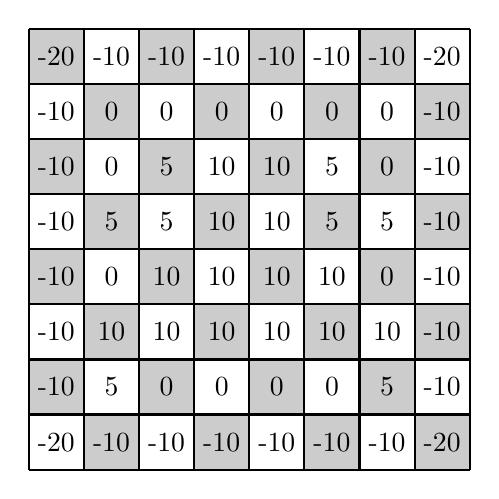
\begin{tikzpicture}[scale=0.7]
        % Draw the chessboard
        \foreach \x in {0,1,...,7} {
            \foreach \y in {0,1,...,7} {
                \pgfmathparse{mod(\x+\y,2) ? "black!20" : "white"}
                \edef\col{\pgfmathresult}
                \fill[\col] (\x,\y) rectangle (\x+1,\y+1);
            }
        }

        % Add the values to the squares
        \node at (0.5,7.5) {-20}; \node at (1.5,7.5) {-10}; \node at (2.5,7.5) {-10}; \node at (3.5,7.5) {-10};
        \node at (4.5,7.5) {-10}; \node at (5.5,7.5) {-10}; \node at (6.5,7.5) {-10}; \node at (7.5,7.5) {-20};

        \node at (0.5,6.5) {-10}; \node at (1.5,6.5) {0}; \node at (2.5,6.5) {0}; \node at (3.5,6.5) {0};
        \node at (4.5,6.5) {0}; \node at (5.5,6.5) {0}; \node at (6.5,6.5) {0}; \node at (7.5,6.5) {-10};

        \node at (0.5,5.5) {-10}; \node at (1.5,5.5) {0}; \node at (2.5,5.5) {5}; \node at (3.5,5.5) {10};
        \node at (4.5,5.5) {10}; \node at (5.5,5.5) {5}; \node at (6.5,5.5) {0}; \node at (7.5,5.5) {-10};

        \node at (0.5,4.5) {-10}; \node at (1.5,4.5) {5}; \node at (2.5,4.5) {5}; \node at (3.5,4.5) {10};
        \node at (4.5,4.5) {10}; \node at (5.5,4.5) {5}; \node at (6.5,4.5) {5}; \node at (7.5,4.5) {-10};

        \node at (0.5,3.5) {-10}; \node at (1.5,3.5) {0}; \node at (2.5,3.5) {10}; \node at (3.5,3.5) {10};
        \node at (4.5,3.5) {10}; \node at (5.5,3.5) {10}; \node at (6.5,3.5) {0}; \node at (7.5,3.5) {-10};

        \node at (0.5,2.5) {-10}; \node at (1.5,2.5) {10}; \node at (2.5,2.5) {10}; \node at (3.5,2.5) {10};
        \node at (4.5,2.5) {10}; \node at (5.5,2.5) {10}; \node at (6.5,2.5) {10}; \node at (7.5,2.5) {-10};

        \node at (0.5,1.5) {-10}; \node at (1.5,1.5) {5}; \node at (2.5,1.5) {0}; \node at (3.5,1.5) {0};
        \node at (4.5,1.5) {0}; \node at (5.5,1.5) {0}; \node at (6.5,1.5) {5}; \node at (7.5,1.5) {-10};

        \node at (0.5,0.5) {-20}; \node at (1.5,0.5) {-10}; \node at (2.5,0.5) {-10}; \node at (3.5,0.5) {-10};
        \node at (4.5,0.5) {-10}; \node at (5.5,0.5) {-10}; \node at (6.5,0.5) {-10}; \node at (7.5,0.5) {-20};

        % Draw the grid
        \draw[thick] (0,0) grid (8,8);
    \end{tikzpicture}
    \caption*{Piece Square Table for the bishop.}\label{fig:piece-square-values-bishop}
\end{figure}

\subsection*{Tapered evaluation}

A chess game typically consists of three phases: the opening, where pieces are developed to more effective squares; the middlegame, where tactical and strategic battles take place; and the endgame, where usually the pawns aim to promote and the side that has the advantage tries to corner the enemy king to mate it.

\vspace{1em}

\noindent It is clearly suboptimal to assign the same piece-square table (PST) bonuses to pieces like the pawn or king during both the middlegame and the endgame. To address this, we implement \textit{tapered evaluation}, a technique that computes two separate evaluations, one for the middlegame/opening and another for the endgame, then interpolates between the two scores to produce a final evaluation~\cite{TaperedEvaluation}.

\vspace{1em}

\noindent First we calculate the percentage of middlegame and the percentage of endgame:

\begin{enumerate}
    \item 100\% Middlegame: The position includes at least all of the initial minor pieces (2 bishops and 2 knights per side), 2 rooks per side, and both queens.
    \item 100\% Endgame: there are zero minor pieces, zero rooks and zero queens.
\end{enumerate}

\noindent The final tapered evaluation score is computed as a weighted average of the middlegame and endgame evaluations. This is formalized in the following equation:
\begin{equation*}
    \text{Eval(position)} = \alpha \cdot \text{middlegameEval} + (1 - \alpha) \cdot \text{endgameEval}
\end{equation*}

\noindent Where $\alpha$ represents the proportion of middlegame.

\vspace{1em}

\noindent We now need two PST's for each piece, in the following~\cref{fig:taperedPSTpawns} there is an example of the middlegame bonus and the endgame bonus for the pawn, as we can see, the pawns in the endgame receive a bonus for being near the promotion squares.

\begin{figure}[H]
    \centering
    \begin{minipage}{0.4\textwidth}
        \centering
        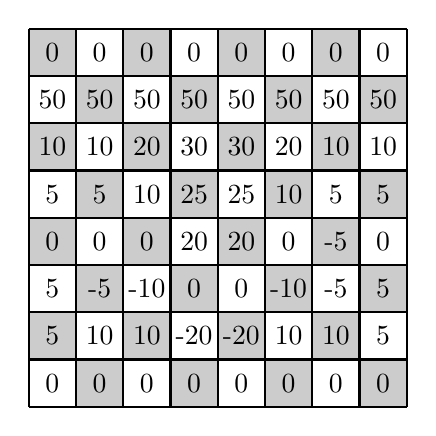
\begin{tikzpicture}[scale=0.6]

            \foreach \x in {0,1,...,7} {
                \foreach \y in {0,1,...,7} {
                    \pgfmathparse{mod(\x+\y,2) ? "black!20" : "white"}
                    \edef\col{\pgfmathresult}
                    \fill[\col] (\x,\y) rectangle (\x+1,\y+1);
                }
            }

            \node at (0.5,7.5) {0};   \node at (1.5,7.5) {0};   \node at (2.5,7.5) {0};   \node at (3.5,7.5) {0};
            \node at (4.5,7.5) {0};   \node at (5.5,7.5) {0};   \node at (6.5,7.5) {0};   \node at (7.5,7.5) {0};

            \node at (0.5,6.5) {50};  \node at (1.5,6.5) {50};  \node at (2.5,6.5) {50};  \node at (3.5,6.5) {50};
            \node at (4.5,6.5) {50};  \node at (5.5,6.5) {50};  \node at (6.5,6.5) {50};  \node at (7.5,6.5) {50};

            \node at (0.5,5.5) {10};  \node at (1.5,5.5) {10};  \node at (2.5,5.5) {20};  \node at (3.5,5.5) {30};
            \node at (4.5,5.5) {30};  \node at (5.5,5.5) {20};  \node at (6.5,5.5) {10};  \node at (7.5,5.5) {10};

            \node at (0.5,4.5) {5};   \node at (1.5,4.5) {5};   \node at (2.5,4.5) {10};  \node at (3.5,4.5) {25};
            \node at (4.5,4.5) {25};  \node at (5.5,4.5) {10};  \node at (6.5,4.5) {5};   \node at (7.5,4.5) {5};

            \node at (0.5,3.5) {0};   \node at (1.5,3.5) {0};   \node at (2.5,3.5) {0};   \node at (3.5,3.5) {20};
            \node at (4.5,3.5) {20};  \node at (5.5,3.5) {0};   \node at (6.5,3.5) {-5};  \node at (7.5,3.5) {0};

            \node at (0.5,2.5) {5};   \node at (1.5,2.5) {-5};  \node at (2.5,2.5) {-10}; \node at (3.5,2.5) {0};
            \node at (4.5,2.5) {0};   \node at (5.5,2.5) {-10}; \node at (6.5,2.5) {-5};  \node at (7.5,2.5) {5};
            
            \node at (0.5,1.5) {5};   \node at (1.5,1.5) {10};  \node at (2.5,1.5) {10};  \node at (3.5,1.5) {-20};
            \node at (4.5,1.5) {-20}; \node at (5.5,1.5) {10};  \node at (6.5,1.5) {10};  \node at (7.5,1.5) {5};

            \node at (0.5,0.5) {0};   \node at (1.5,0.5) {0};   \node at (2.5,0.5) {0};   \node at (3.5,0.5) {0};
            \node at (4.5,0.5) {0};   \node at (5.5,0.5) {0};   \node at (6.5,0.5) {0};   \node at (7.5,0.5) {0};

            \draw[thick] (0,0) grid (8,8);
        \end{tikzpicture}
        \caption*{Pawn middlegame PST}
    \end{minipage}
    \hfill
    \begin{minipage}{0.4\textwidth}
        \centering
        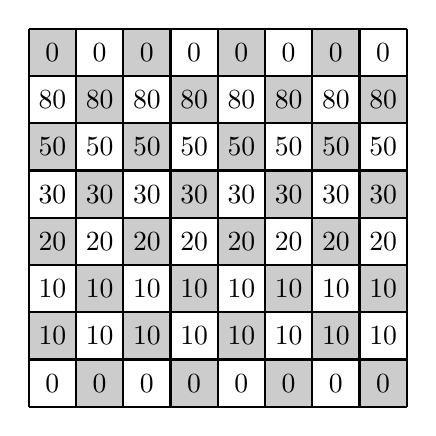
\begin{tikzpicture}[scale=0.6]

            \foreach \x in {0,1,...,7} {
                \foreach \y in {0,1,...,7} {
                    \pgfmathparse{mod(\x+\y,2) ? "black!20" : "white"}
                    \edef\col{\pgfmathresult}
                    \fill[\col] (\x,\y) rectangle (\x+1,\y+1);
                }
            }

            \node at (0.5,7.5) {0}; \node at (1.5,7.5) {0}; \node at (2.5,7.5) {0}; \node at (3.5,7.5) {0};
            \node at (4.5,7.5) {0}; \node at (5.5,7.5) {0}; \node at (6.5,7.5) {0}; \node at (7.5,7.5) {0};

            \node at (0.5,6.5) {80}; \node at (1.5,6.5) {80}; \node at (2.5,6.5) {80}; \node at (3.5,6.5) {80};
            \node at (4.5,6.5) {80}; \node at (5.5,6.5) {80}; \node at (6.5,6.5) {80}; \node at (7.5,6.5) {80};

            \node at (0.5,5.5) {50}; \node at (1.5,5.5) {50}; \node at (2.5,5.5) {50}; \node at (3.5,5.5) {50};
            \node at (4.5,5.5) {50}; \node at (5.5,5.5) {50}; \node at (6.5,5.5) {50}; \node at (7.5,5.5) {50};

            \node at (0.5,4.5) {30}; \node at (1.5,4.5) {30}; \node at (2.5,4.5) {30}; \node at (3.5,4.5) {30};
            \node at (4.5,4.5) {30}; \node at (5.5,4.5) {30}; \node at (6.5,4.5) {30}; \node at (7.5,4.5) {30};

            \node at (0.5,3.5) {20}; \node at (1.5,3.5) {20}; \node at (2.5,3.5) {20}; \node at (3.5,3.5) {20};
            \node at (4.5,3.5) {20}; \node at (5.5,3.5) {20}; \node at (6.5,3.5) {20}; \node at (7.5,3.5) {20};

            \node at (0.5,2.5) {10}; \node at (1.5,2.5) {10}; \node at (2.5,2.5) {10}; \node at (3.5,2.5) {10};
            \node at (4.5,2.5) {10}; \node at (5.5,2.5) {10}; \node at (6.5,2.5) {10}; \node at (7.5,2.5) {10};

            \node at (0.5,1.5) {10}; \node at (1.5,1.5) {10}; \node at (2.5,1.5) {10}; \node at (3.5,1.5) {10};
            \node at (4.5,1.5) {10}; \node at (5.5,1.5) {10}; \node at (6.5,1.5) {10}; \node at (7.5,1.5) {10};

            \node at (0.5,0.5) {0}; \node at (1.5,0.5) {0}; \node at (2.5,0.5) {0}; \node at (3.5,0.5) {0};
            \node at (4.5,0.5) {0}; \node at (5.5,0.5) {0}; \node at (6.5,0.5) {0}; \node at (7.5,0.5) {0};

            \draw[thick] (0,0) grid (8,8);
        \end{tikzpicture}
        \caption*{Pawn endgame PST}
    \end{minipage}
    \caption{Tapered Piece Square Tables for pawn.}\label{fig:taperedPSTpawns}
\end{figure}

\newpage

\section{Move generator}
\label{sec:moveGenerator}

Calculating the legal moves in a chess position is a more difficult and tedious task
than it might seem, mainly due to the unintuitive rules of \textit{en passant} and castling,
and it is also difficult to restrict the moves of pinned pieces~\cite{GenerateLegalMovesEfficiently}.

\vspace{1em}

\noindent The full implementation of the move generator can be found in\\ \texttt{src\textbackslash{}move\_generator\textbackslash{}move\_generator\_basic.cpp}.

\vspace{1em}

\noindent Our move generator uses bitboard operations to quickly and efficiently compute all legal moves available in any given chess position.

\subsection*{Precomputed attacks}

\noindent The first step is to precompute attack patterns for each piece type on every square of the board. These patterns are stored as bitboards, typically in arrays indexed by both piece type and square.

\vspace{1em}

\noindent For instance, the image below illustrates the precomputed attack bitboard for a bishop positioned on the $d4$ square.

\begin{figure}[H]
    \centering
    \newchessgame
    \chessboard[
        showmover=false,
        setfen=8/8/8/8/3B4/8/8/8 w - - 0 1,
        markstyle=border,
        color=blue, markfields={a1,b2,c3,e5,f6,g7,h8,g1,f2,e3,c5,b6,a7}
    ]
    \caption*{Precomputed attack for the bishop on the d4 square.}\label{fig:precomputedAttackBishop}
\end{figure}

\subsection*{Bitboard of danger squares}

Using the previously precomputed attack patterns, we generate a bitboard representing all the squares currently attacked by the waiting side (the side not having the move). This bitboard is referred to as the danger bitboard. It includes all squares that are unsafe for the king of the side to move, as moving the king to any of these squares would result in an illegal position.~\cref{fig:BitboardDangers} illustrates an example of this concept.

\begin{figure}[H]
    \centering
    \begin{minipage}{0.4\textwidth}
        \centering
        \newchessgame
        \chessboard[
            showmover=true,
            setfen=n7/2p5/5kP1/5P2/1R3K2/r7/8/8 w - - 0 1
        ]
        \caption*{White is the side to move.}
    \end{minipage}
    \hfill
    \begin{minipage}{0.35\textwidth}
        \centering
        \includegraphics[width=1.0\textwidth]{Imagenes/bitboardDangers.png}
        \caption*{Danger bitboard for the black (waiting) side.}        
    \end{minipage}
    \caption{Example of a danger bitboard squares attacked by the black side.}\label{fig:BitboardDangers}
\end{figure}

\noindent The danger bitboard is constructed by performing a bitwise OR operation across all legal attacks from the opponent's pieces. For non-sliding pieces such as pawns, knights, and kings, their legal attack bitboards match exactly with their precomputed attack patterns.

\vspace{1em}

\noindent However, sliding pieces as rooks, bishops, and queens require additional handling. Their attacks depend on the presence of blockers in their movement paths.~\cref{fig:blockerExample} shows an example where the attacks of sliding pieces are limited due to blocking pawns. In this case, the rook sliding attack is being blocked by the pawns.

\begin{figure}[H]
    \centering
    \newchessgame
    \chessboard[
        showmover=true,
        setfen=8/8/3r2p1/8/3P4/8/8/8 w - - 0 1,
        markstyle=border,
        color=blue, markfields={d7,d8,d5,c6,b6,a6,e6,f6},
        color=red, markfields={d4,g6}
    ]
    \caption{Example of blocking pieces.}\label{fig:blockerExample}

\end{figure}

\noindent Currently, calculating legal attacks for sliding pieces involves iterating along orthogonal and diagonal directions until a blocking piece is encountered. This approach is relatively inefficient. In subsequent sections, we present optimization techniques that address this issue.

\subsection*{Bitboard of pinned pieces}

\noindent The next challenging aspect of legal move generation is handling pinned pieces. A pinned piece cannot move freely, as doing so would expose its king to check, making the move illegal. An example of a pinned piece is shown in~\cref{fig:pinnedPiece}.

\begin{figure}[H]
    \centering
    \newchessgame
    \chessboard[
        showmover=true,
        setfen=3r4/8/8/8/3N4/8/3K4/8 w - - 0 11
    ]
    \caption{The black rook pins the white knight. If the knight moves, the white king could be captured, making the move illegal.}\label{fig:pinnedPiece}
\end{figure}

\noindent We must compute a bitboard that contains all pinned pieces on the board. This allows us to restrict their movement accordingly during move generation. However, identifying pinned pieces is computationally expensive, as it requires iterating through the attack patterns of sliding pieces and checking for alignment with the king and potential blockers.

\subsection*{Capture and push mask}

\noindent The final bitboards required for handling checks are the \textit{capture mask} and the \textit{push mask}. The capture mask identifies the squares occupied by the checking pieces, while the push mask includes the squares in between the king and the checking piece along the line of attack.

\begin{center}
    \centering
    \newchessgame
    \chessboard[
        showmover=true,
        setfen=8/8/5N2/2K4r/8/8/8/8 w - - 0 1,
        markstyle=border,
        color=blue, markfields={d5,e5,f5,g5},
        color=red, markfields={h5}
    ]
\end{center}

\noindent The capture mask is shown in red, and the push mask is shown in blue.

\vspace{1em}

\noindent These masks are applied during check situations. In such cases, the only legal responses are:

\begin{itemize}[itemsep=1pt]
    \item Capturing the checking piece (a move to a square in the capture mask).
    \item Blocking the check (a move to a square in the push mask).
    \item Moving the king to a safe square outside the danger bitboard.
\end{itemize}

\subsection*{Legal move computation}

\noindent The final step is to calculate the legal moves of the side to move using the previously calculated information: bitboard of attacks, dangers, pinned pieces, and push and capture masks.

\vspace{1em}

\noindent We begin by determining the number of checking pieces, which can be deduced from the number of bits set in the capture mask. Based on this, three main scenarios must be handled:

\begin{itemize}[itemsep=1pt]
    \item \textit{Double check}: If there are two or more checkers, the only legal option is to move the king to a square that is not under attack, outside the danger bitboard. No other piece can legally move in this case.
    \item \textit{No check}: In the absence of any checks, we iterate through all the pieces belonging to the side to move and generate their legal moves. If a piece is pinned (inside pinned piece bitboard), its movement is constrained to the direction of the pin.
    \item \textit{Single check}: If exactly one checker is present, we again iterate over all pieces. The moves available are to capture the checker (captures inside the capture mask), to block the check (moves inside the push mask), or to move the king to a legal square.
\end{itemize}

\noindent Finally, the special moves of castling and \textit{en passant} are handled explicitly by looking for the castling rights and the \textit{en passant} target square in the game state.

\subsection*{Testing the move generator: perft test}

To ensure the correctness of our move generator, we perform what is known as a \textit{Perft test} (performance test, move path enumeration)~\cite{Perft}.

\vspace{1em}

\noindent Perft is a debugging function in which we generate the entire game tree for a specific position up to a given depth and count all the resulting nodes. We can then compare our results with those of other engines, such as \textit{Stockfish}. Since \textit{Stockfish} is widely regarded as highly accurate, it serves as a reliable reference for validating move generation.

\vspace{1em}

\noindent In~\cref{tab:perftResults}, we present our Perft results alongside those of \textit{Stockfish} for seven well-known test positions at depth 6. The identical node counts in all cases confirm the correctness of our move generator.

\begin{table}[H]
    \centering
    \begin{tabular}{|l|r|l|}
    \hline
    \textit{FEN NAME} & \textit{Stockfish Nodes} & \textit{AlphaDeepChess Nodes} \\
    \hline
    \texttt{FEN KIWIPETE}       &  8031647685 &  8031647685   \\
    \texttt{FEN EDWARDS2}       &  6923051137 &  6923051137   \\
    \texttt{FEN STRANGEMOVES}   &  5160619771 &  5160619771   \\
    \texttt{FEN TALKCHESS}      &  3048196529 &  3048196529   \\
    \texttt{FEN TEST4}          &  706045033  &  706045033    \\
    \texttt{FEN TEST4 MIRROR}   &  706045033  &  706045033    \\
    \texttt{FEN START POS}      &  119060324  &  119060324    \\
    \hline
    \end{tabular}
    \caption{Perft results at depth 6: comparison between \textit{Stockfish} and \textit{AlphaDeepChess}~\cite{PerftResults}.}\label{tab:perftResults}
\end{table}

\section{Move ordering}\label{cap:moveOrdering}
Once having explained the move generator function, in this chapter we detail the implementation of the move ordering heuristic.

\vspace{1em}

\noindent \parbox{\textwidth}{The complete implementation can be found in\\\texttt{src\textbackslash{}move\_ordering\textbackslash{}move\_ordering\_MVV\_LVA.cpp}.}

\vspace{1em}

\noindent During the search process, the earlier we explore the best move in a position, the better the algorithm performs. In the best-case scenario, if the first move explored is indeed the optimal one, the remaining branches of the tree can be pruned. To achieve this, we sort the legal moves by estimated quality, from best to worst~\cite{MoveOrdering}.

\subsection*{Most valuable victim - least valuable aggressor}

The heuristic we implemented is the \textit{Most Valuable Victim - Least Valuable Aggressor (MVV-LVA)}. In this approach, a move receives a high score if it captures a valuable piece using a less valuable one. For example, capturing a queen with a pawn is considered a very strong move~\cite{MVVLVA}.

\vspace{1em}

\noindent We implemented this heuristic using a look-up table indexed by the moving piece and the captured piece, as shown in~\cref{tab:mvv-lva-table}. Capturing a queen with a pawn receives a score of 55, while doing the opposite receives 11 points.

\begin{table}[H]
    \centering
    \begin{tabular}{|c|r|r|r|r|r|r|}
        \hline
        \textit{Victim $\backslash$ Attacker} & \textit{P} & \textit{N} & \textit{B} & \textit{R} & \textit{Q} & \textit{K} \\
        \hline
        \textit{P}     & 15 & 14 & 13 & 12 & 11 & 10 \\
        \hline
        \textit{N}     & 25 & 24 & 23 & 22 & 21 & 20 \\
        \hline
        \textit{B}     & 35 & 34 & 33 & 32 & 31 & 30 \\
        \hline
        \textit{R}     & 45 & 44 & 43 & 42 & 41 & 40 \\
        \hline
        \textit{Q}     & 55 & 54 & 53 & 52 & 51 & 50 \\
        \hline
        \textit{K}     &  0 &  0 &  0 &  0 &  0 &  0 \\
        \hline
    \end{tabular}
    \caption{MVV-LVA heuristic table: Rows = Victims, Columns = Attackers.}\label{tab:mvv-lva-table}
\end{table}

\subsection*{Killer moves}

The main limitation of MVV-LVA is that it only applies to capture moves. In fact, assigning meaningful scores to non-capturing (quiet) moves is a challenging task. To address this, we implemented the \textit{killer move} heuristic, which assigns high scores to certain quiet moves.

\vspace{1em}

\noindent A \textit{killer move} is a quiet, non-capturing move which can cause a cutoff in different branches of the tree at the same depth~\cite{KillerMoves}.

\begin{figure}[H]
    \centering
    \newchessgame
    \chessboard[
        showmover=false,
        setfen=1r3k2/ppp2ppp/1n1bp3/q2p2N1/3P4/2P1P3/PP3PPP/2BQ2KR w K - 0 3,
        pgfstyle=straightmove, color=blue,
        markmoves={d1-h5},
        arrow=to,
        markstyle=circle,
        color=red, markfields={f7}
    ]
    \caption{Killer move example.}\label{fig:killer_move_example}
\end{figure}

\noindent In~\cref{fig:killer_move_example}, the queen moves to h5, threatening checkmate on f7. This quiet move prunes all other moves that do not respond to the threat.

\vspace{1em}

\noindent These moves are remembered and prioritized during move ordering, as they have proven effective in position at the same depth in the search tree. We implemented a table where we store two moves that causes a cutoff per search depth. There could be more than two killer moves, our replacement policy is to always maintain the older killer move found in one slot, and in the other slot store the least recently found.

\vspace{1em}

\noindent If a quiet move being evaluated matches one of the killer moves stored at the current search depth, we increase its score by 70 points. This value is chosen to ensure that killer moves are prioritized above most quiet moves, but still allow the most valuable captures (according to the MVV-LVA heuristic) to take precedence when appropriate. This balance helps improve pruning efficiency without overlooking critical tactical opportunities.